\documentclass[11pt, a4paper]{article}
\usepackage{pdfpages}
\usepackage{parallel}
\usepackage[T2A]{fontenc}
\usepackage{ucs}
\usepackage[utf8x]{inputenc}
\usepackage[polish,english,russian]{babel}
\usepackage{hyperref}
\usepackage{rotating}
\usepackage[inner=2cm,top=1.8cm,outer=2cm,bottom=2.3cm,nohead]{geometry}
\usepackage{listings}
\usepackage{graphicx}
\usepackage{wrapfig}
\usepackage{longtable}
\usepackage{indentfirst}
\usepackage{array}
\usepackage{tikzsymbols}
\usepackage{soul}
\usepackage[ruled,vlined]{algorithm2e}
%\counterwithout{figure}{section} 

\usepackage{url}
\makeatletter
\g@addto@macro{\UrlBreaks}{\UrlOrds}
\makeatother

\newcolumntype{P}[1]{>{\raggedright\arraybackslash}p{#1}}
\frenchspacing
\usepackage{fixltx2e} %text sub- and superscripts
\usepackage{icomma} % коскі ў матэматычным рэжыме
\PreloadUnicodePage{4}

\newcommand{\longpage}{\enlargethispage{\baselineskip}}
\newcommand{\shortpage}{\enlargethispage{-\baselineskip}}

\def\switchlang#1{\expandafter\csname switchlang#1\endcsname}
\def\switchlangbe{
\let\saverefname=\refname%
\def\refname{Літаратура}%
\def\figurename{Іл.}%
}
\def\switchlangen{
\let\saverefname=\refname%
\def\refname{References}%
\def\figurename{Fig.}%
}
\def\switchlangru{
\let\saverefname=\refname%
\let\savefigurename=\figurename%
\def\refname{Литература}%
\def\figurename{Рис.}%
}

\hyphenation{admi-ni-stra-tive}
\hyphenation{ex-pe-ri-ence}
\hyphenation{fle-xi-bi-li-ty}
\hyphenation{Py-thon}
\hyphenation{ma-the-ma-ti-cal}
\hyphenation{re-ported}
\hyphenation{imp-le-menta-tions}
\hyphenation{pro-vides}
\hyphenation{en-gi-neering}
\hyphenation{com-pa-ti-bi-li-ty}
\hyphenation{im-pos-sible}
\hyphenation{desk-top}
\hyphenation{elec-tro-nic}
\hyphenation{com-pa-ny}
\hyphenation{de-ve-lop-ment}
\hyphenation{de-ve-loping}
\hyphenation{de-ve-lop}
\hyphenation{da-ta-ba-se}
\hyphenation{plat-forms}
\hyphenation{or-ga-ni-za-tion}
\hyphenation{pro-gramming}
\hyphenation{in-stru-ments}
\hyphenation{Li-nux}
\hyphenation{sour-ce}
\hyphenation{en-vi-ron-ment}
\hyphenation{Te-le-pathy}
\hyphenation{Li-nux-ov-ka}
\hyphenation{Open-BSD}
\hyphenation{Free-BSD}
\hyphenation{men-ti-on-ed}
\hyphenation{app-li-ca-tion}

\def\progref!#1!{\texttt{#1}}
\renewcommand{\arraystretch}{2} %Іначай формулы ў матрыцы зліпаюцца з лініямі
\usepackage{array}

\def\interview #1 (#2), #3, #4, #5\par{

\section[#1, #3, #4]{#1 -- #3, #4}
\def\qname{LVEE}
\def\aname{#1}
\def\q ##1\par{{\noindent \bf \qname: ##1 }\par}
\def\a{{\noindent \bf \aname: } \def\qname{L}\def\aname{#2}}
}

\def\interview* #1 (#2), #3, #4, #5\par{

\section*{#1\\{\small\rm #3, #4. #5}}
\ifx\ParallelWhichBox\undefined%
    \addcontentsline{toc}{section}{#1, #3, #4}%
\else%
\ifnum\ParallelWhichBox=0%
    \addcontentsline{toc}{section}{#1, #3, #4}%
\fi\fi%

\def\qname{LVEE}
\def\aname{#1}
\def\q ##1\par{{\noindent \bf \qname: ##1 }\par}
\def\a{{\noindent \bf \aname: } \def\qname{L}\def\aname{#2}}
}

\newcommand{\interviewfooter}[1]{
\vskip 1em
\noindent \textit{#1}
}


\begin{document}

\title{1995 "--- Трекбол Logitech TrackMan Marble}
\date{}
\maketitle

Данный трекбол имеет 3 клавиши, отвечаюие за стандартные функции кнопок мыши, и шар, предназначенный для вращения большим пальцем правой руки (рис. \ref{fig:trackman}). Драйвер позволял использовать для прокрутки вращение шара с зажатой средней кнопкой (при нажатии эта кнопка выполняет привычную функцию), но следует отметить, что сущестовала также модификация этого трекбола с традиционным колесом прокрутки в вырезе третьей кнопки.
Трекбол подключается к компьютеру по интерфейсу PS/2.

Корпус трекбола имеет постоянный наклон вправо, благодаря чему запястье лежащей на трекболе руки находится в более естественном положении (рис. \ref{fig:trackmanHand}). В то время, как шар прокручивается большим пальцем, остальные пальцы работают так же, как при пользовании обычной мышью, что делает конструкцию более привлекательной для пользователя, привыкшего к мыши или попеременно работающего мышью и трекболом. Но она имеет и свои недостатки: подвижность большого пальца несколько меньше, что отражается на быстроте и точности позиционирования, к тому же такая конструкция, в отличие от «классической», совершенно непригодна для левшей.

\begin{figure}[h]
    \centering
    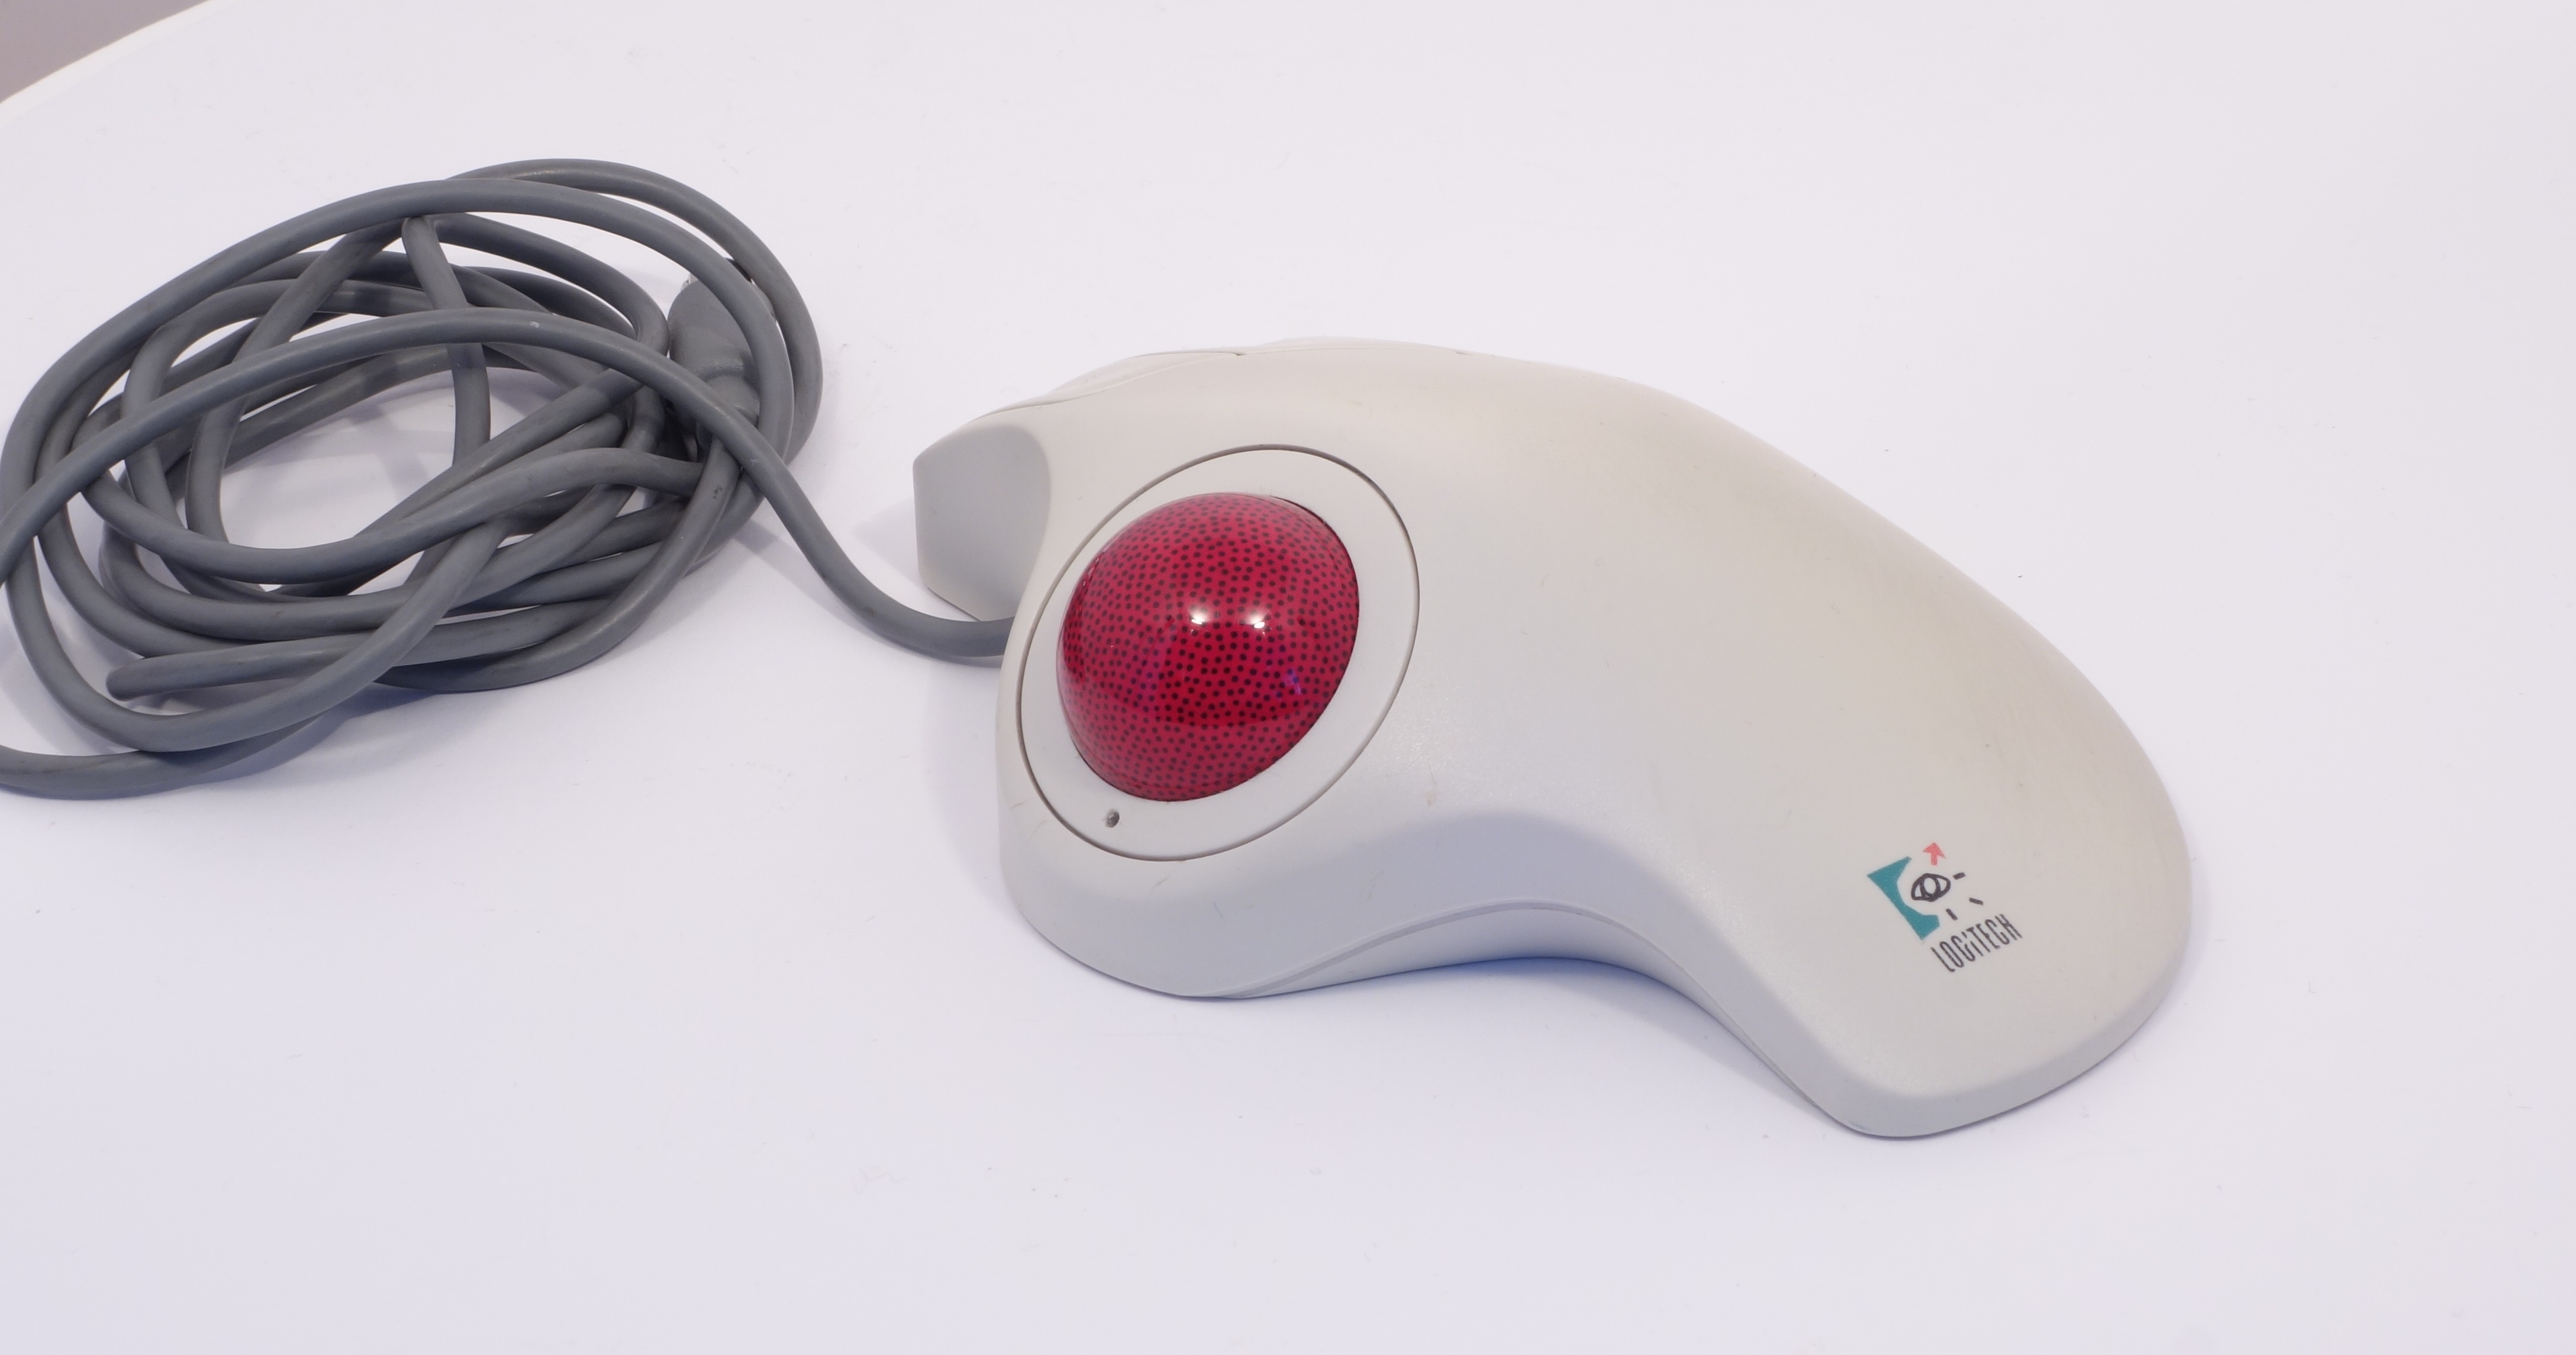
\includegraphics[scale=0.3]{1995_logitech_trackman/2.15.JPG}
    \caption{Изображение Logitech TrackMan}
    \label{fig:trackman}
\end{figure}

\begin{figure}[h]
    \centering
    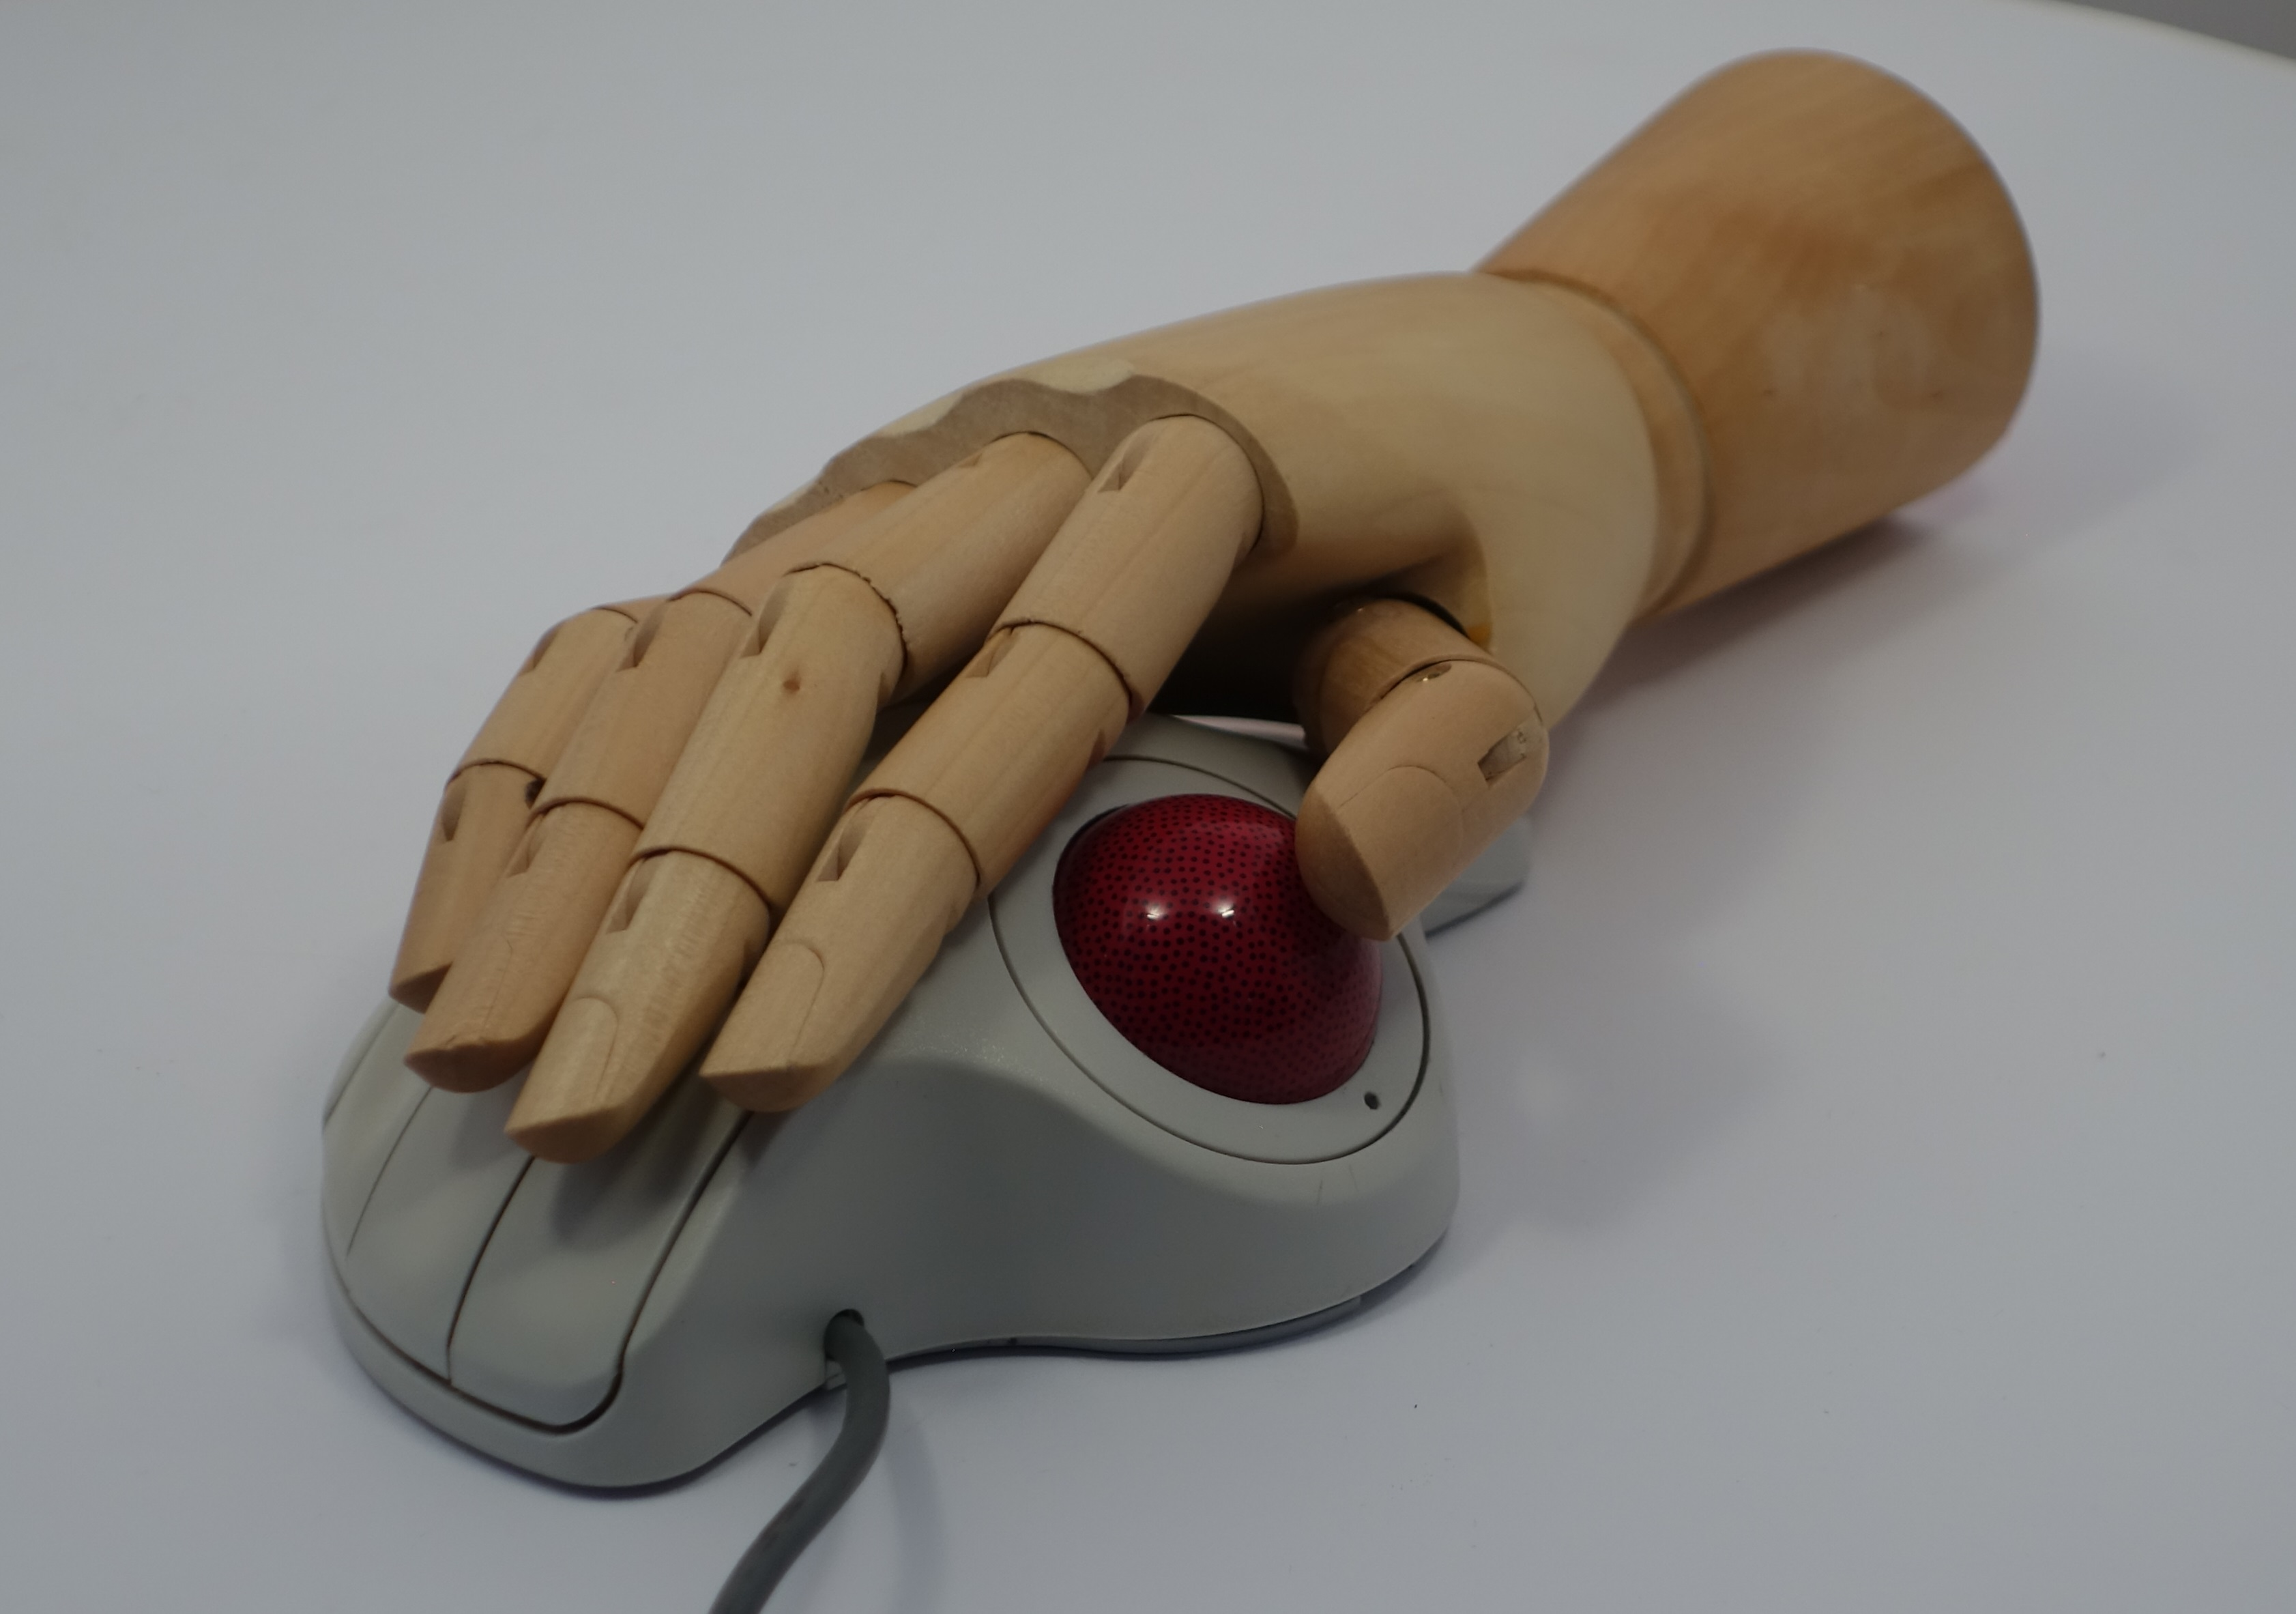
\includegraphics[scale=0.5]{1995_logitech_trackman/2.14.JPG}
    \caption{Изображение Logitech TrackMan с моделью руки человека}
    \label{fig:trackmanHand}
\end{figure}

Из особенностей можно отметить нестандартный рисунок шара, на котором нанесен регулярный узор из тёмных точек. Разбор трекбола (рис. \ref{fig:trackmanInside}) показывает, что причиной этой расцветки является отказ фирмы Logitech от традиционной схемы оптомеханической мыши в пользу аналога оптической мыши, считывающей изменения яркости с помощью специального коврика с нанесенной на нём сеткой. Только в данном случае роль коврика играет рисунок на вращающемся шаре. По заверениям разработчика, распознавание движения реализовано системой на основе искусственной нейронной сети \cite{marbleAdv}.

\begin{figure}[h]
    \centering
    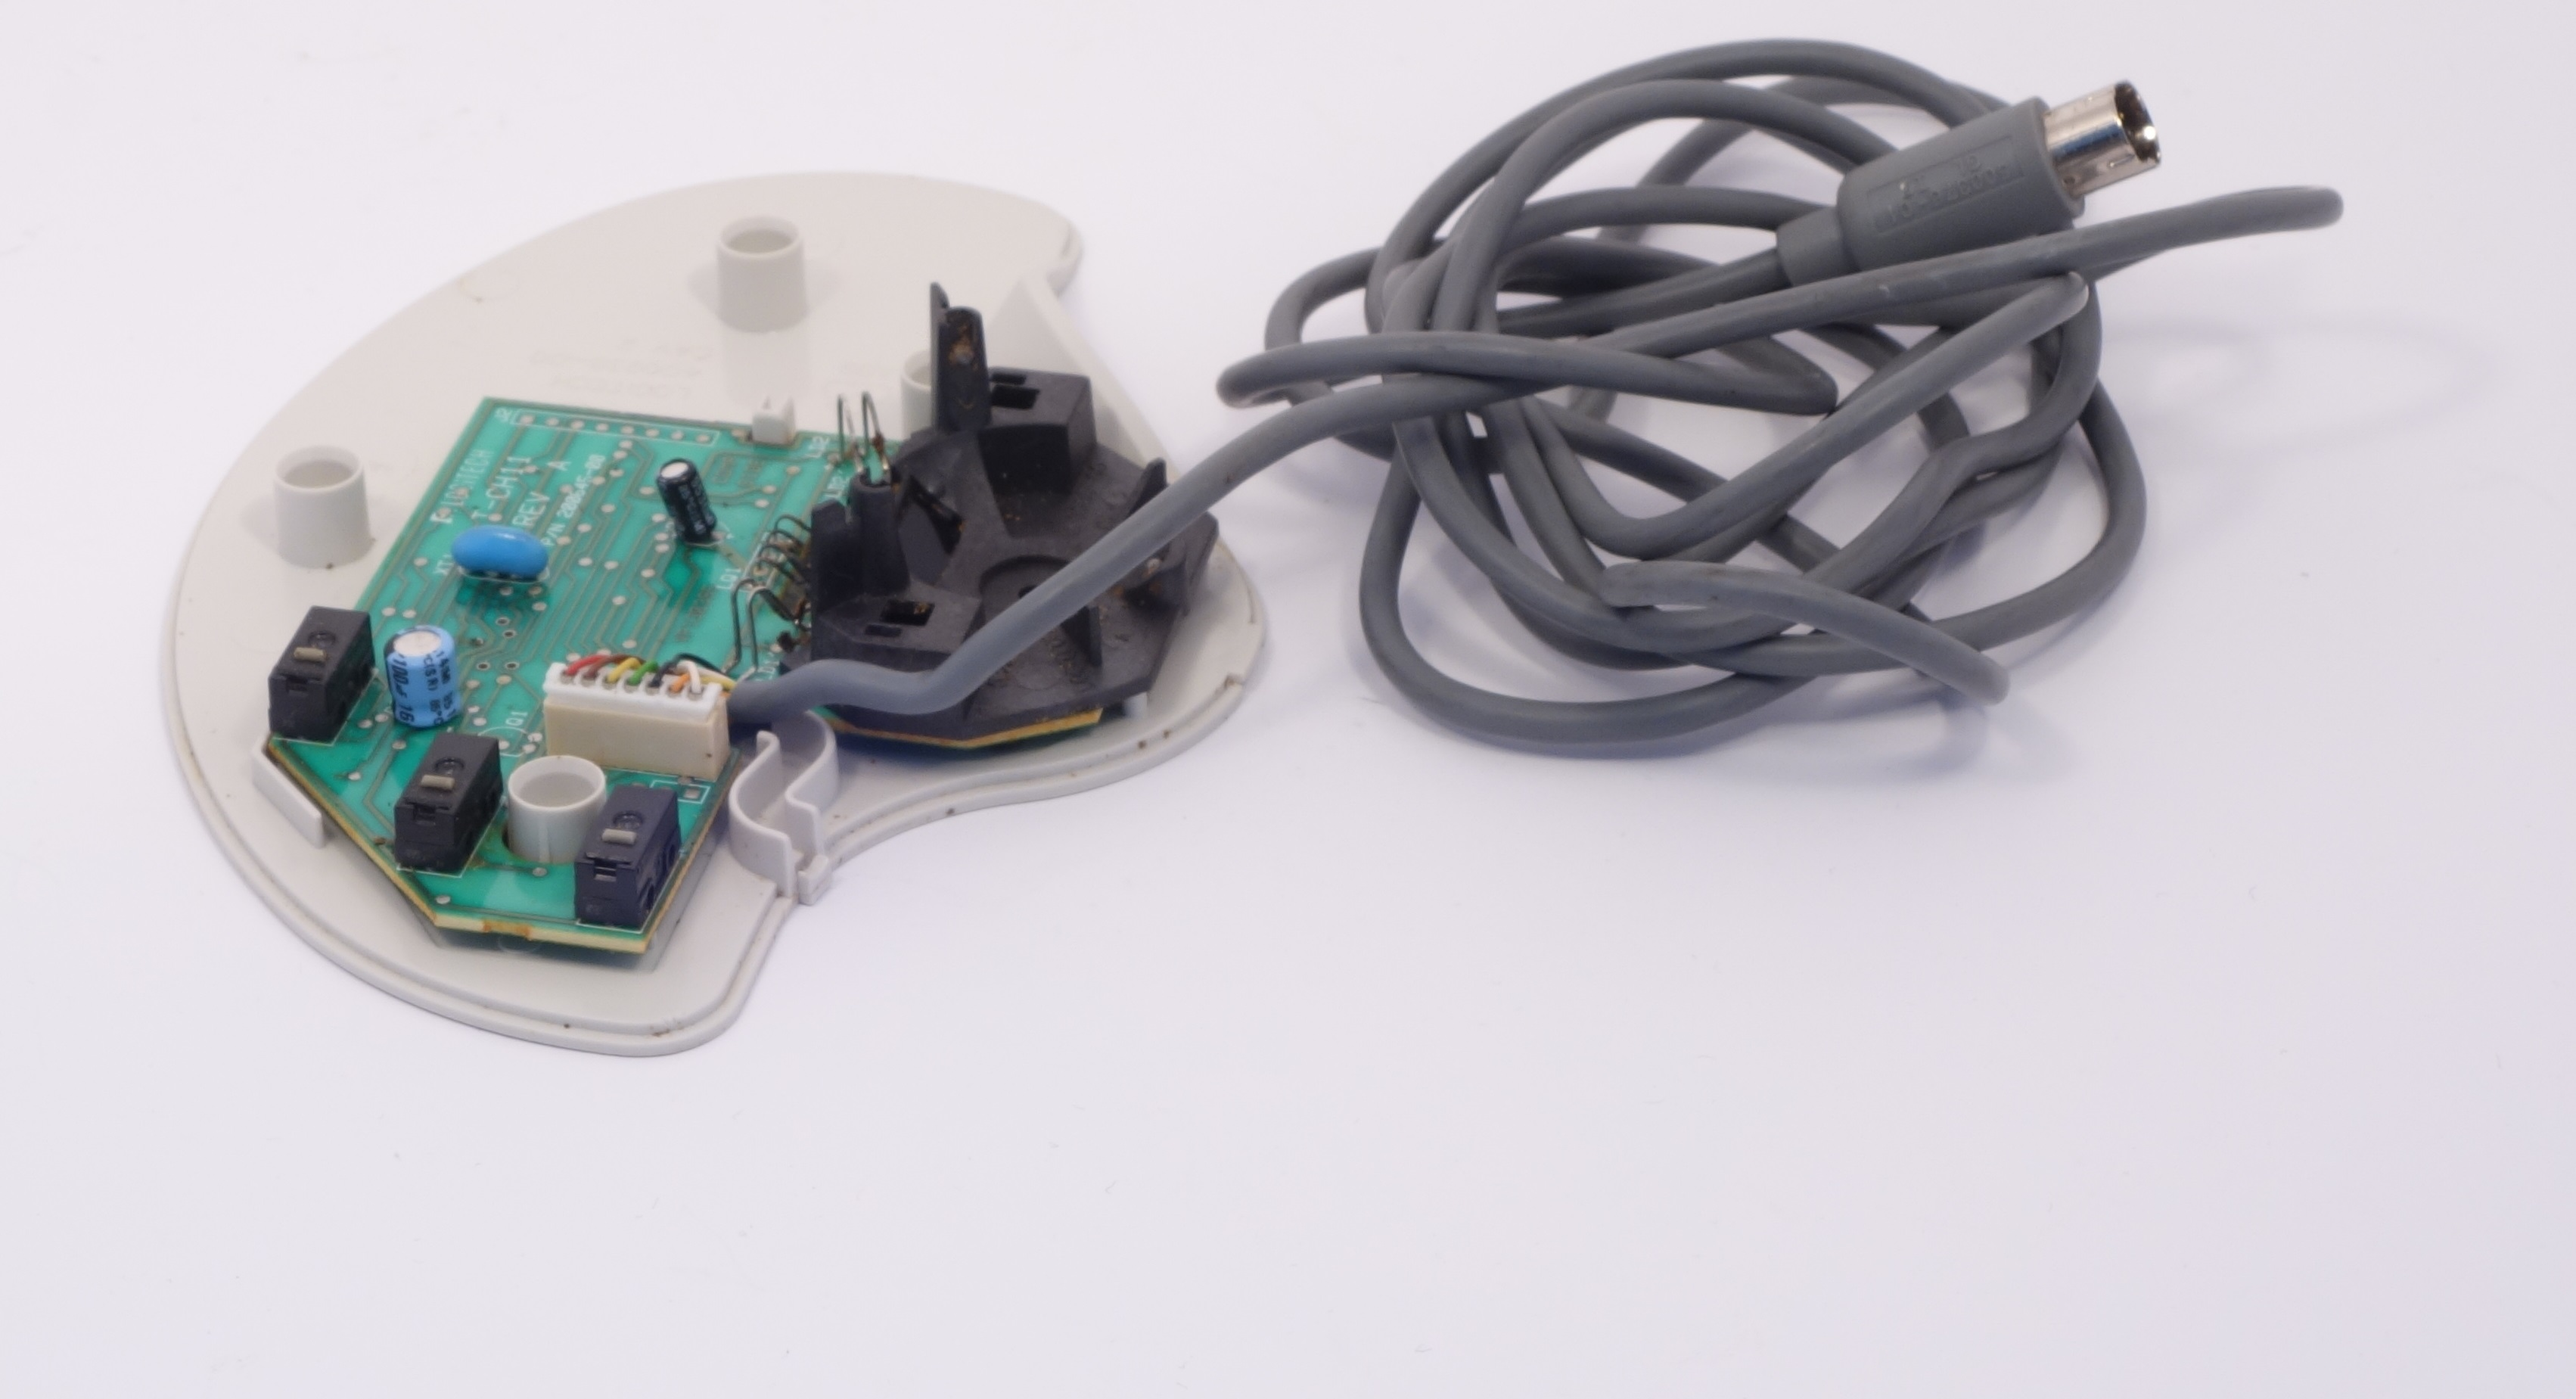
\includegraphics[scale=0.5]{1995_logitech_trackman/201.JPG}
    \caption{Изображение Logitech TrackMan изнутри}
    \label{fig:trackmanInside}
\end{figure}

\begin{figure}[h]
    \centering
    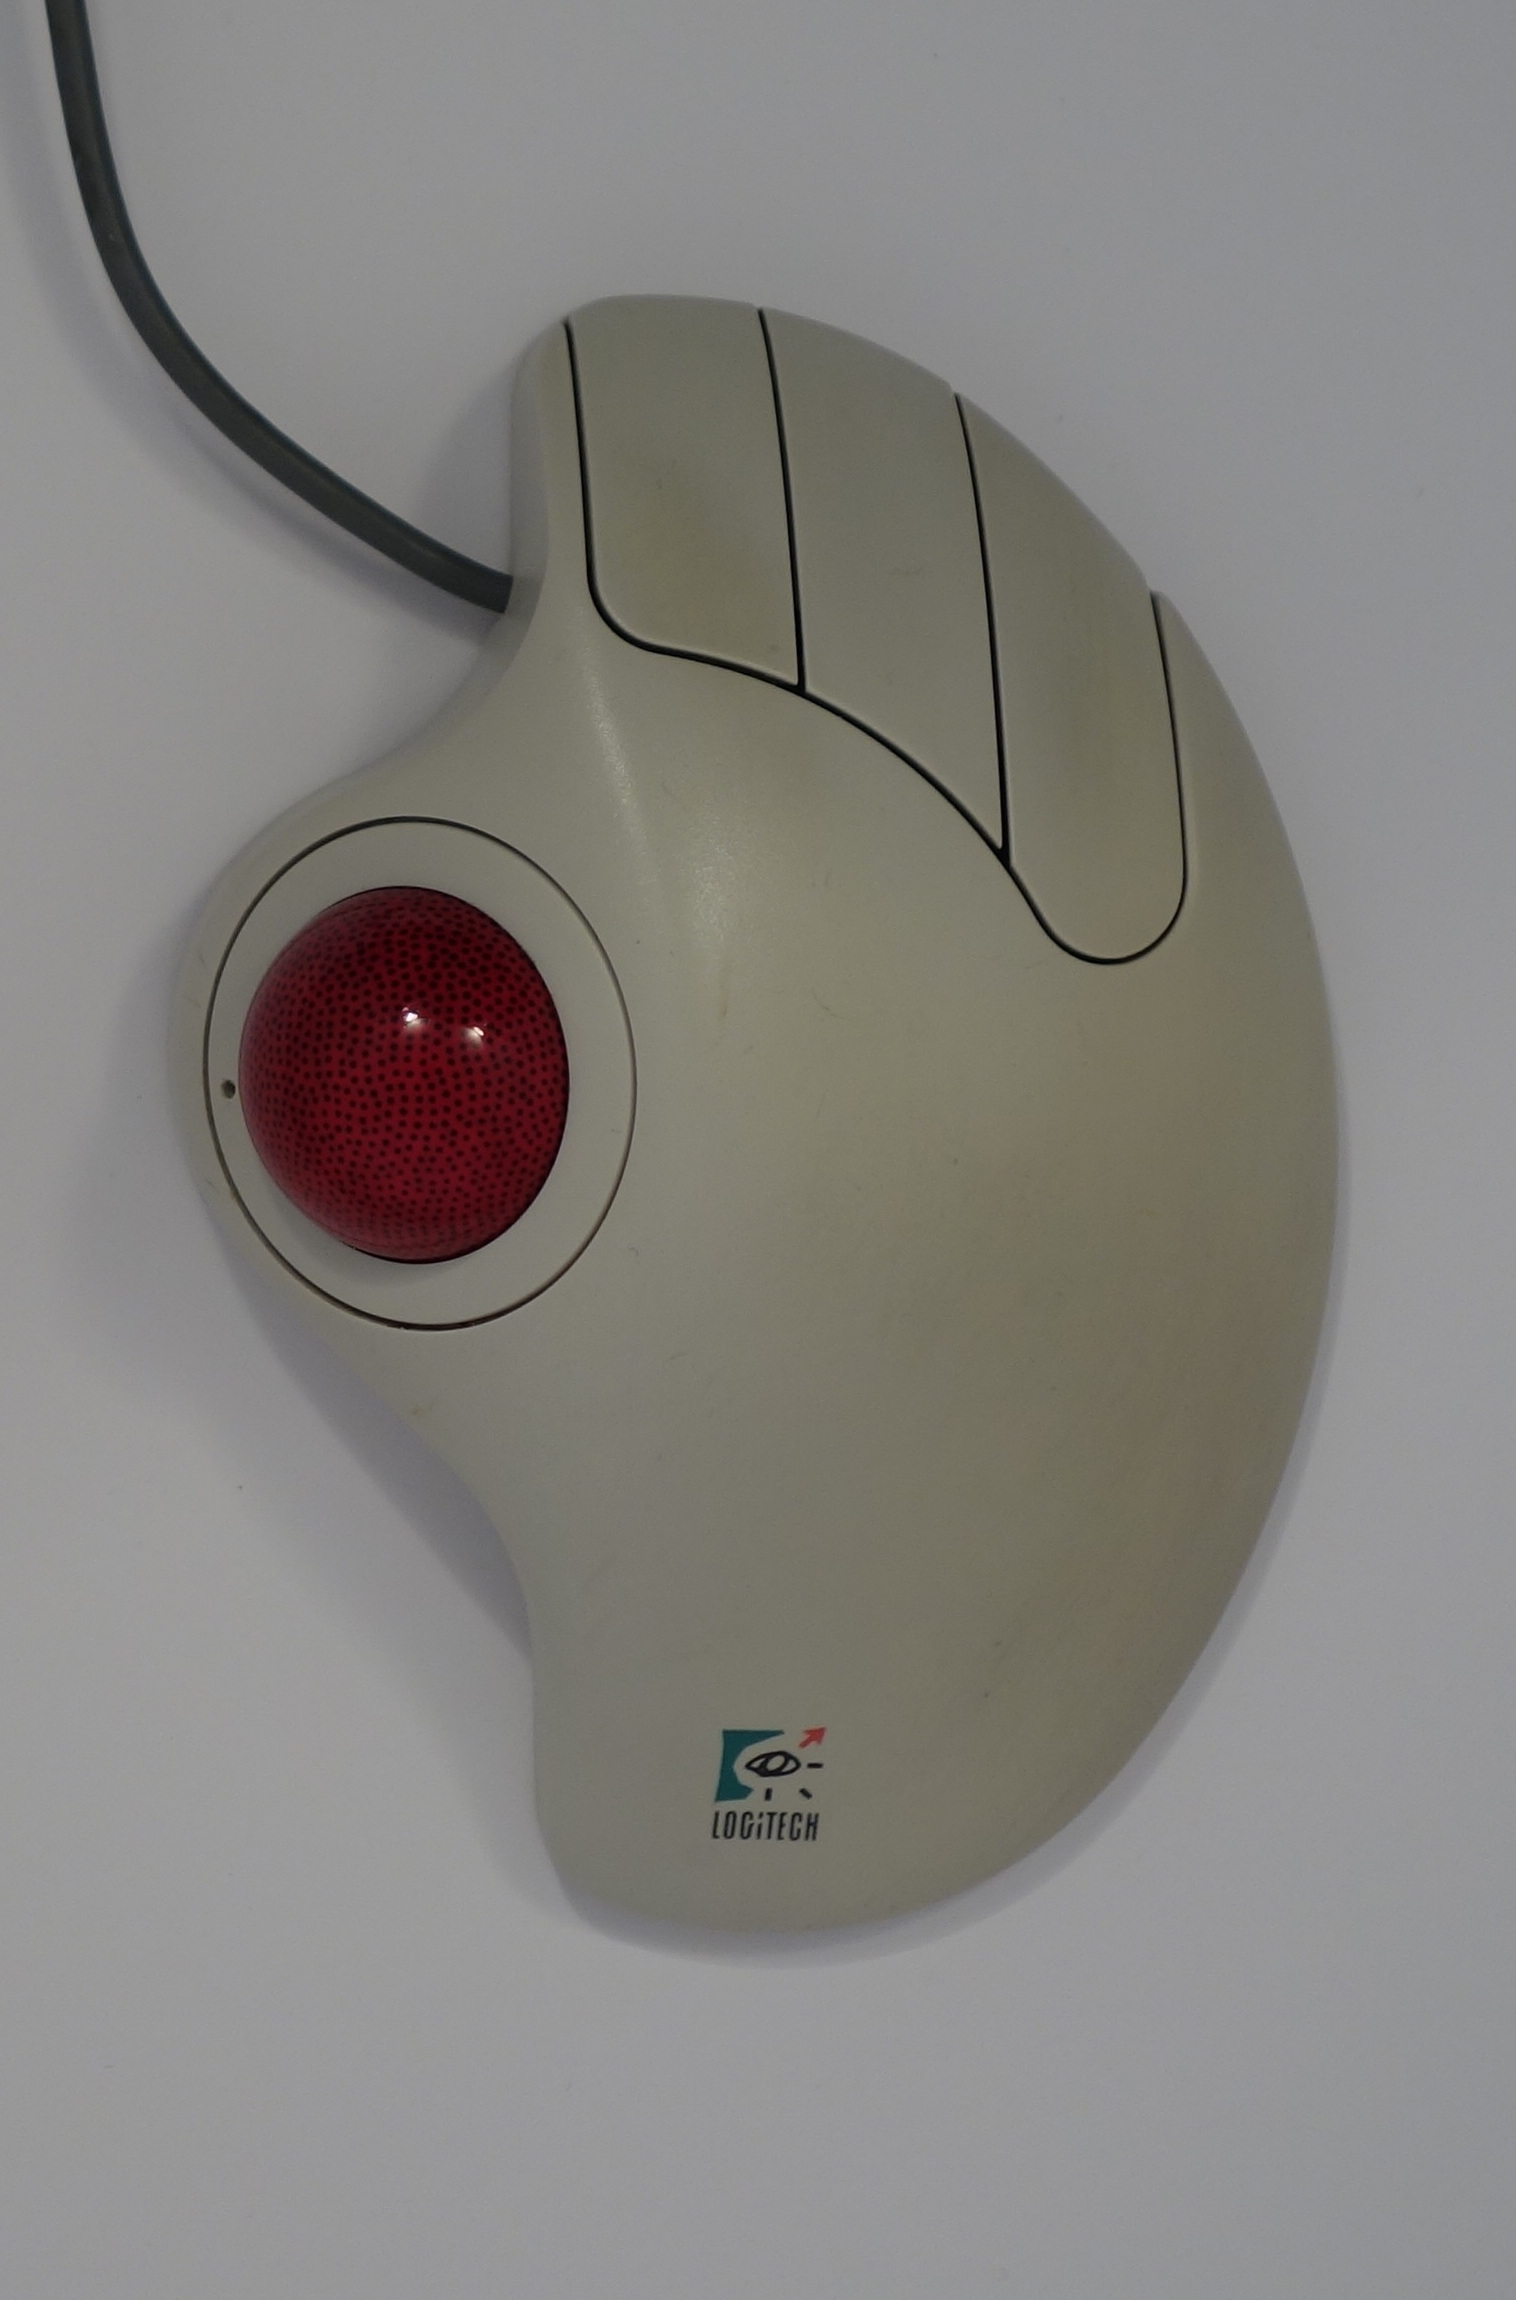
\includegraphics[scale=1]{1995_logitech_trackman/2.16.JPG}
    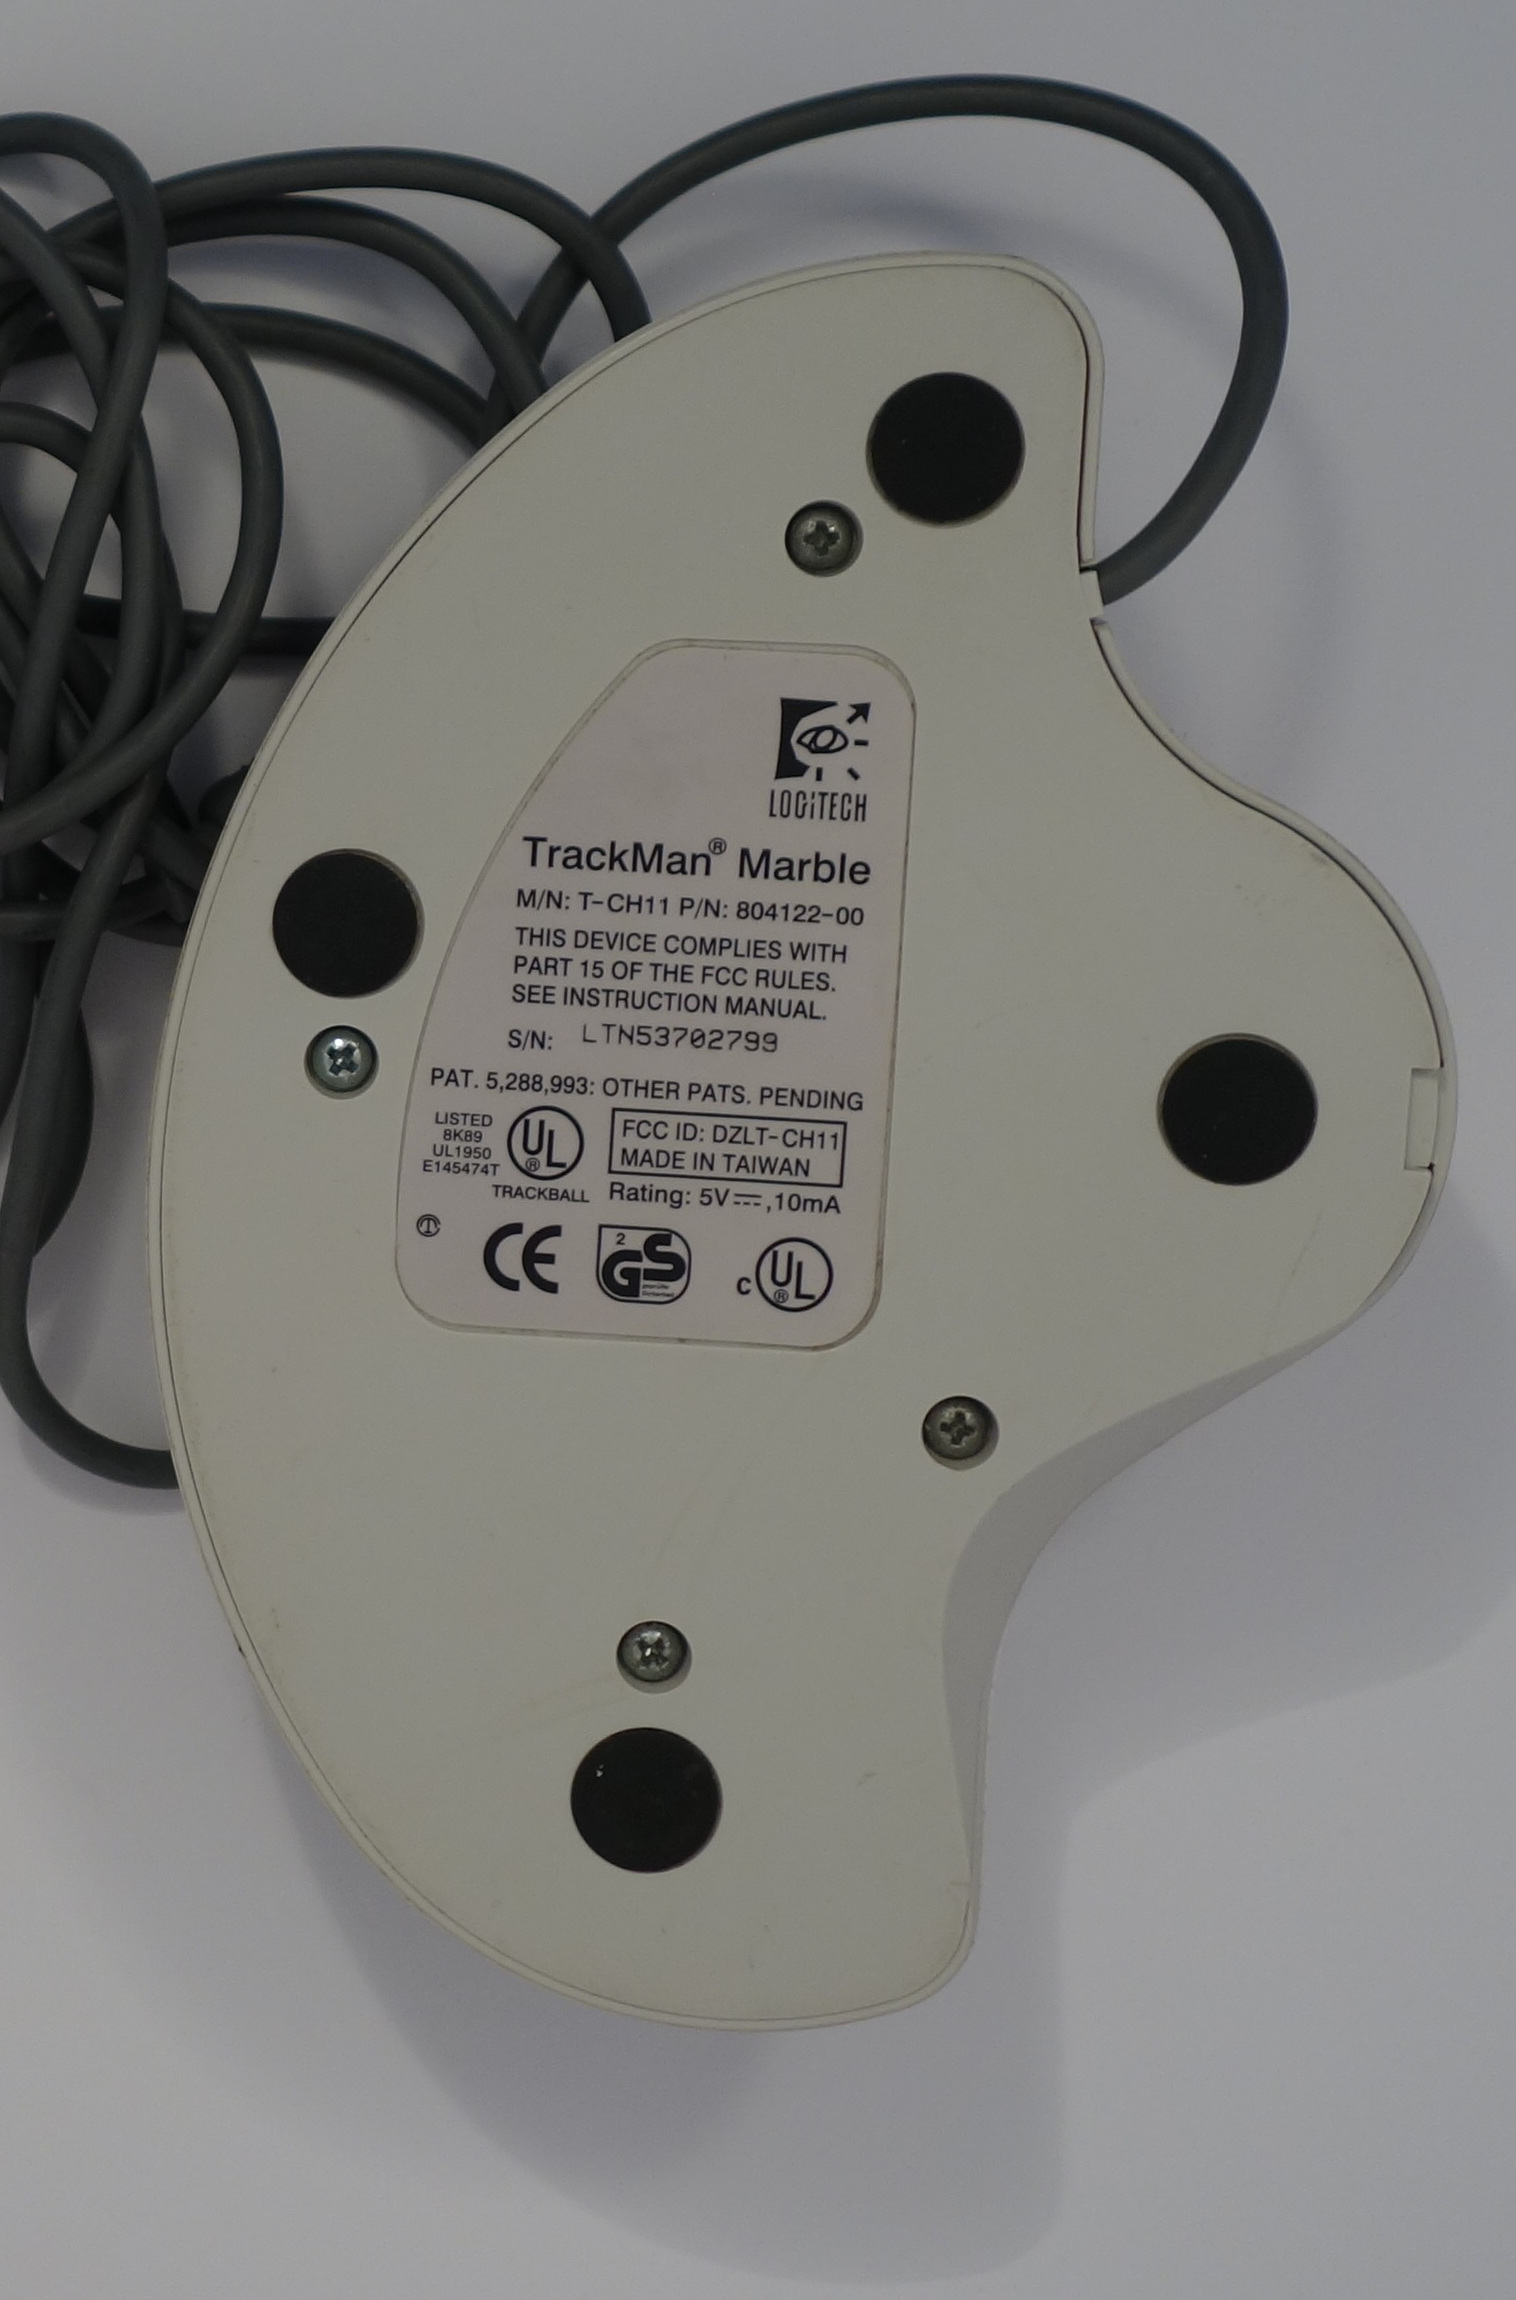
\includegraphics[scale=1]{1995_logitech_trackman/2.17.JPG}
    \caption{Изображение Logitech TrackMan, вид сверху и снизу}
    \label{fig:trackmanTopAndBottom}
\end{figure}
    
    Маркировка на нижней части трекбола содержит код FCC ID (рис. \ref{fig:trackmanTopAndBottom}).
    Проверка кода по базе данных Федеральной комиссии по коммуникациям США показывает, что трекбол был разработан компанией Logitech в 1995 году.

%\begin{figure}[h]
%    \centering
%    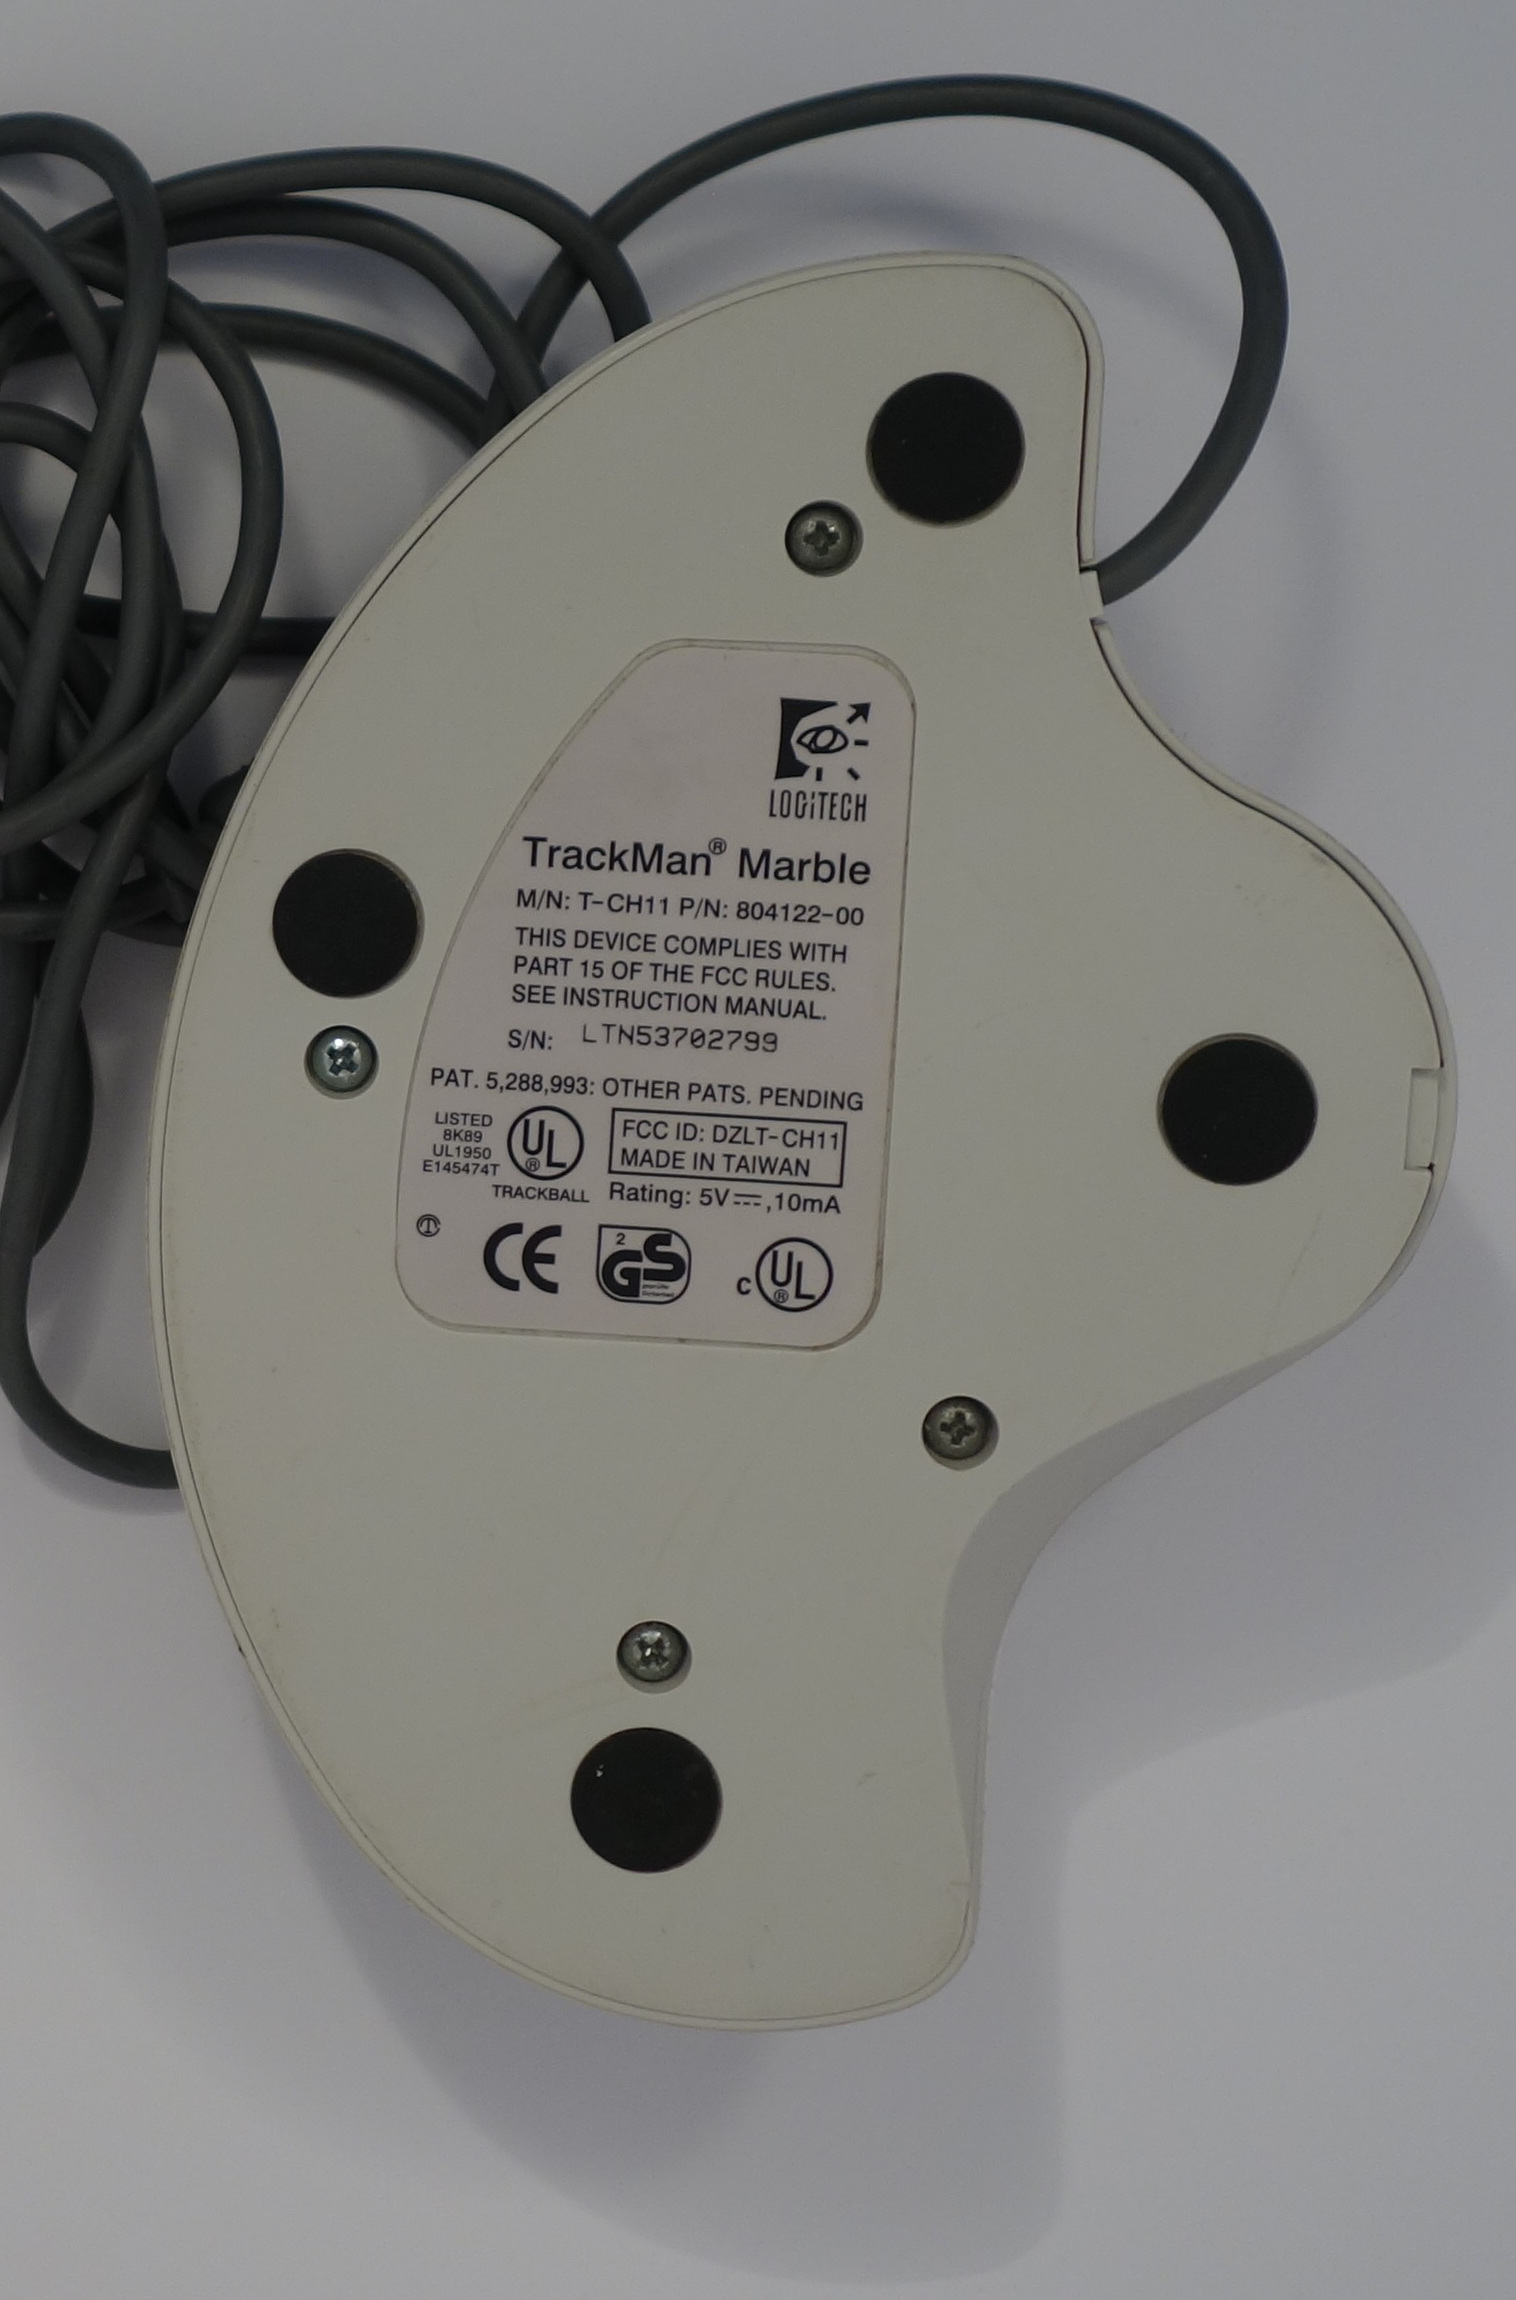
\includegraphics[scale=0.5]{1995_logitech_trackman/2.17.JPG}
%    \caption{Изображение Logitech TrackMan вид снизу}
%    \label{fig:trackmanBottom}
%\end{figure}

\begin{thebibliography}{9}
\bibitem{marbleAdv} Melissa J. Perenson. New \& improved. News of announced products and upgrades. // PC Magazine, Vol. 14, No. 22. -- December 19, 1995. -- p. 61 -- 66.
\end{thebibliography}

\end{document}
